\documentclass[french,a4paper, 12pt]{article}

\usepackage[utf8]{inputenc}
\usepackage[T1]{fontenc}

\usepackage{geometry}
\usepackage{graphicx}
\usepackage{xspace}
\usepackage{parskip}
\usepackage{amssymb}

\usepackage[french]{babel}

\geometry{verbose,tmargin=1in,bmargin=1in,lmargin=0.7in,rmargin=0.7in}

\title{\textbf{Oraux des ENS}}
\author{Samuel Gallay}

\begin{document}
\maketitle

\section*{Physique (LCR)}

45 minutes, pas de préparation : On considère un condensateur cylindrique de hauteur $L$ dirigé selon l'axe $e_z$ avec le bas du condensateur en $z = 0$, de rayons intérieur et extérieurs $r_1$ et $r_2$. On se place dans l'ARQS, la charge dépendant du temps, et on demande d'abord de calculer la puissance dissipée (ie le flux du vecteur de Poynting) à travers la surface $z = L$.

J'ai commencé par dire des choses intelligentes, mais l'examinateur s'est rendu compte que je ne comprennais rien à l'ARQS, donc j'ai eu le droit à de nombreuses questions de cours. D'abord qu'est-ce que le vecteur nabla ? Remontrez moi l'équation de D'Alembert pour le champ électrique. Qu'est-ce que l'ARQS? En fait j'ai confondu au début  les deux courants dans l'équation de Maxwell-Ampère. J'ai dû expliquer ce qui se passait physiquement dans un condensateur, et je n'y arrivais pas. L'examinateur, par ailleurs très sympathique, notait les bêtises que je disais, et me faisait me contredire pour que je comprenne ce qu'il se passait. Distances caractériqtiques de l'ARQS, etc...

Bon, je suis très déçu de moi sur ce coup là, d'habitude j'arrive à sauver les meubles pendant mes oraux de physique...

\section*{Mathématiques (U)}
Qu'est-ce que c'était mieux que mon oral de physique !

Démonstration sympathique du théorème de Cayley-Hamilton : prenez $A \in M_n(C)$ et $P\in C[X]$ le polynôme caractéristique de $A$, et calculez de deux manières différentes, pour $r$ assez grand, l'intégrale matricielle (coefficients par coefficients) $$I = \int_0^{2\pi} r e^{i\theta}P(re^{i\theta})(A-re^{i\theta}I_n)^{-1}d\theta$$ 

Je conseille de le chercher un peu tout seul... L'examinateur était au début assez sec et l'élève avant moi m'a souhaité bon courage avec une tête terrorisée. Il ne fallait juste pas se laisser démonter, il m'a donné des indications régulièrement, quand je bloquais. Il m'a surtout signalé les petites erreurs de calcul (j'en ai fait trop souvent). L'oral à commencé en retard et terminé en avance... j'ai le sentiment que l'examinateur avait déjà une certaine lassitude des oraux, j'étais le dernier de la journée.

Quelques indications (essayez sans, ça doit être à peu près possible d'avancer seul). D'abord pour $r$ grand $(A - re^{i\theta})$ est inversible car le polynôme caractéristique possède un nombre fini de racines. Ensuite, pour le premier calcul de I, on considère P comme un polynôme quelconque. On factorise par $-re^{i\theta}$ le terme matriciel, on l'écrit comme une série entière. J'ai dû discuter avec la norme triple : définition, pourquoi ai-je choisi celle-là... On inverse la série et l'intégrale : on l'a fait un peu vite à mon goût, mais la somme des intégrales des normes des fonctions de $\theta$ convergent. On calcule l'intégrale, d'abord le cas des monômes, linéarité, et on trouve $2\pi P(A)$ (j'ai un doute sur le signe, mais on se fiche un peu de la constante). Pour le second calcul de $I$, définition du polynôme caractéristique, comatrice, et calcul coefficient par coefficient (l'intégrale est matricielle). Le déterminant qui apparait dans les coefficients de la comatrice est un polynôme en $e^{i\theta}$. Donc l'intérieur des intégrales coeff par coeff sont des polynômes en $e^{i\theta}$ dont le coefficient constant est nul. Par un des calculs précédent $I = 0$.

\section*{TIPE (ULCR)}

L'oral s'est très bien passé, j'avais deux examinateurs, un homme et une femme. Le monsieur connaissait assez bien le langage Prolog (pari gagné !). Je pense qu'ils avaient parcouru assez vite mon rapport, mais ils s'y étaient intéressés. L'oral s'est déroulé comme une alternance d'exposé et de questions. J'avais un diaporama, et ils avaient le rapport sous les yeux. Certaines questions étaient posées pour me tester comme \emph{qu'est-ce que vous pouvez me dire sur les grammaires ? Non contextuelles ? LL(1) ? Compilation vers un automate ?} Des questions sur les choix de la représentation des données, des parcours... D'autres questions étaient plutôt de la curiosité : \emph{J'aime beaucoup le Prolog, mais pourquoi avez vous décidé de travailler sur Prolog ?} Des discussions sur la compilation de Prolog, et sur différentes extensions : le \emph{cut} (ça allait) et sur la métaprogrammation avec les \emph{assert}. Là je n'y connsissais rien, mais il fallait souligner la difficulté de compiler le assert par rapport à l'interpréter...

\section*{Informatique (LCR)}

Je suis très déçu de cet oral d'informatique. C'est avec celui-ci que je jouais mon admission aux ENS de Saclay et Rennes, le coefficient étant bien plus élevé que celui de physique par exemple, et j'ai perdu (je n'ai rien fait seul dans le sujet, et je devais paraître ralenti...) J'avais révisé des sujets, cela ne m'a servi à rien. J'espère que l'info d'Ulm sera plus intéressante.

L'oral consiste en 30 minutes de préparation et 30 minutes de passage. On considère un ensemble $A$ possèdant une loi associative et commutative (notée multiplicativement), et on s'intéresse au calcul des puissance d'un élément $x$ de cet ensemble.

Pour formaliser le coût du calcul, on s'autorise deux règles de production sur une partie $\Gamma$ de $A$. La première produit l'élément $x$ à partir de $\varnothing$. La seconde prend deux éléments de $x^i$ et $x^j$ dans $\Gamma$ et produit $\Gamma \cup \{x^{i+j}\}$

Exemple d'un calcul de $x^7$ avec ce formalisme :

$$\varnothing \longrightarrow \{x\}\longrightarrow \{x, x^2\} \longrightarrow \{x, x^2, x^4\}\longrightarrow \{x, x^2, x^4, x^6\}\longrightarrow \{x, x^2, x^4, x^6, x^7\}$$

On définit le coût de calcul $C(n)$ de $x^n$ comme le nombre minimal de flèches nécessaires pour créer $x^n$ à partir de $\varnothing$. Avec cet exemple, $C(7) \le 5$.

Les questions. Montrez que $C(n) \le n$. Montrez que $C(n) \le 2\lfloor \log_2{n}  \rfloor$.

Déjà cette question était mal fichue, cette inégalité n'est pas vraie pour des petits entiers, comme 7 par exemple (si je ne me plante pas)... Ce n'est pas une très grosse erreur d'énoncé, mais c'est embêtant si on veut initialiser une récurrence, ou si on cherche des exemples sur des petits entiers... Un sujet de concours ne devrait pas contenir d'erreur, c'est déjà assez de la loterie comme ça !

Montrez que l'algorithme trouvé à la question précedente n'est pas optimal. (L'algo de la question précédente est l'exponentiation rapide, et de mauvais cas sont les $2^n-1$ par exemple.)

Montrez que $\lceil \log_2(n)\rceil \le C(n)$.

Montrez que $C(n)$ est équivalent à $\log_2(n)$ quand $n\rightarrow +\infty$.

Exposez un algorithme utilisant la décomposition en facteurs premiers de $n$. Montrez que cet algorithme peut-être meilleur et moins bon dans une infinité de cas que celui proposé en $2\lfloor \log_2(n) \rfloor$.

On définit ensuite les \emph{power trees} de \textsc{Knuth} et on demande de construire un meilleur algorithme.

\section*{Mathématiques (CR)}

On se place dans un convexe $A$ de $\mathbb{C}$, et on considère une fonction $f$ de $A$ dans $\mathbb{C}$ telle que $$ \lim_{z\rightarrow z_0}{\frac{f(z) - f(z_0)}{z - z_0}} $$ existe. On montre d'abord que $f$ est continue, puis que $f$ est différentiable. Ensuite on considère un chemin continu et $C^1$ par morceaux $\gamma : [a, b] \rightarrow A$, tel que $\gamma(a) = \gamma(b)$. On montre que $$\int_a^bf(\gamma(t))\gamma'(t)dt = 0$$ Enfin, avec les mêmes hypothèses sur $\gamma$, pour $z$ n'appartenant pas à $\gamma([a, b])$, on pose $$I(z)=\frac{1}{2i\pi}\int_a^b\frac{\gamma'(t)}{\gamma(t)-z}dt$$ Montrez que $I(z)\in\mathbb(Z)$.

L'exercice n'était pas très difficile, mais je n'étais pas assez réveillé pour être rapide et efficace. L'examinatrice était très calme, et m'a donné des indications. Pour la dernière question, on peut introduire $\phi : [a, b] \rightarrow \mathbb{C}$ définie par $$\phi(t) = exp(\int_a^t\frac{\gamma'(s)}{\gamma(s)-z}ds)$$
J'aurais dû être plus rapide.

\section*{Anglais (XULCR)}

Difficile de dire si cela s'est bien ou mal passé. Mon anglais n'était pas exceptionnel, et il y a des questions sur la vidéo auxquelles je n'ai pas su répondre, mais dans l'ensemble ça reste comme une colle d'anglais. Il y avait deux examinatrices qui posaient les questions à tour de rôle.

La vidéo venait de la chaîne PBS Terra que l'on trouve sur YouTube, et était sur le Cascadia Earthquake. On la retrouve facilement. Je me souviens que la durée était de 6 minutes et quelques secondes. Je pense que c'étaient les premières 6 minutes et 14 secondes sur YouTube (à 10 sec près en tout cas).

\section*{Informatique (U)}

\section*{TP d'algorithmique (ULCR)}

\section*{Divagations parisiennes}

Il fait chaud dans Paris, surtout dans un studio sous les toits. Il n'y a pas d'insectes et on ne voit pas les étoiles parce que la nuit il fait comme jour dehors.

\section*{Dimanche}

Je suis arrivé à Paris dimanche en début d'après-midi, et j'ai fait une visite complète du 5ième arrondissement. J'ai juste voulu prendre mes premiers repères : la rue Lhomond et la rue d'Ulm, Henri IV, Louis le Grand, le collège de France, le Panthéon, le Luxembourg et le jardin des plantes. J'ai fait des courses, j'aime bien la rue Mouffetard et je loge dans le quartier des Gobelins, ce qui est très pratique pour passer des oraux.

\section*{Lundi}

Après mon oral de physique raté je suis allé faire une sieste. L'oral de maths s'est mieux passé, donc je suis allé me promener. Je suis allé voir Jussieu, Nôtre-Dame, le Louvre, les Tuileries jusqu'à l'obélisque, puis le bord de la Seine jusqu'à la tour Eiffel et le Champ-de-Mars. Je suis rentréen métro : j'ai eu le droit à un panne de courant de la part de la RATP (heureusement j'étais à quai). J'ai pu avoir un apreçu du célèbre esprit lutécien, et j'ai improvisé un itinéraire alternatif.

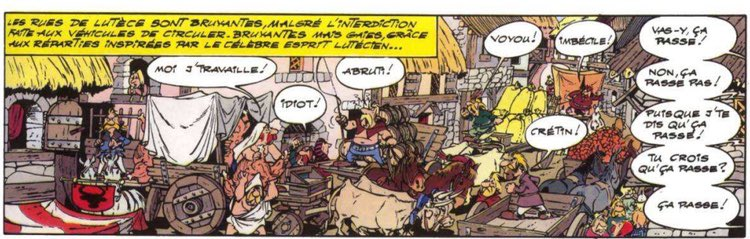
\includegraphics[scale=0.65]{asterix.jpg}

\section*{Mardi}

J'ai passé l'après-midi avec un ami de lycée, qui passe aussi les concours, on est allé manger une glace au jardin des Plantes (il fait vraiment chaud). Le soir mon autre amie de lycée qui me prête généreusement son studio est rentrée à Paris.

\section*{Mercredi}

On est allé mangé au CROUS de Censier pour 1 euro, c'est pas mal. J'ai admiré avec horreur les constructions du plateau de Saclay. Je suis descendu à la station Lozère et je suis monté à l'X. Je voulais voir à quoi tout cela ressemblait. N'allez pas à pieds des écoles X/ENSAE à Centrale/ENS. La ballade prend une petite heure, mais c'est très moche. À vélo ça doit aller (il y a une piste cyclable), mais prenez plutôt le bus comme tout le monde. Je suis rentré dans les bâtiments de centrale, c'est grand mais très vide... Il y a beaucoup de grands bâtiments en travaux sur le plateau. 

\section*{Jeudi}

Je me suis perdu dans l'X. On est allé regarder un film amusant au cinéma du Pnathéon.

\section*{Vendredi}

\end{document}